\section*{Výsledky měření}
Měření proběhlo při pokojové teplotě ($\approx \SI{22}{\degreeCelsius}$).

Jako voltmetr jsme používali METEX M 3860 M a jako ampérmetr MASETECH MY65.
Používáme síťové napětí s frekvencí \SI{50}{\hertz}.

Odporová dekáda měla přesnost \SI{0.1}{\percent} a kondenzátorová dekáda \SI{1}{\percent}.

Osciloskopem jsme změřili špičkové napětí na svorkách sekundárního vinutí transformátoru $U_0=\SI{9.3(3)}{\volt}$ a z něho podle \eqref{e:efektivni} vyplývá efektivní hodnota \SI{6.5(2)}{\volt}.
Chybu odečtu na osciloskopu jsme odhadli na polovinu nejmenšího dílku.

\subsection*{Jednocestný usměrňovač}

Voltmetrem na střídavém rozsahu jsme změřili efektivní napětí \SI{6.66(9)}{\volt}.
Hodnoty z obou přístrojů jsou tedy v dobré shodě.

Měřili jsme jednocestný usměrňovač.
Při hodnotě zatěžovacího odporu \SI{10}{\kilo\ohm} jsme proměřili závislost stejnosměrného napětí $U$ na filtrační kapacitě $C$, výsledky jsou v tabulce \ref{t:kapacita} a v grafu \ref{g:prvni}.
Špičkovou hodnotu pulzního průběhu jsme odečetli na osciloskopu $U_0=\SI{8.5(1)}{\volt}$.

\begin{graph}[htbp] 
\centering
% GNUPLOT: LaTeX picture with Postscript
\begingroup
  \makeatletter
  \providecommand\color[2][]{%
    \GenericError{(gnuplot) \space\space\space\@spaces}{%
      Package color not loaded in conjunction with
      terminal option `colourtext'%
    }{See the gnuplot documentation for explanation.%
    }{Either use 'blacktext' in gnuplot or load the package
      color.sty in LaTeX.}%
    \renewcommand\color[2][]{}%
  }%
  \providecommand\includegraphics[2][]{%
    \GenericError{(gnuplot) \space\space\space\@spaces}{%
      Package graphicx or graphics not loaded%
    }{See the gnuplot documentation for explanation.%
    }{The gnuplot epslatex terminal needs graphicx.sty or graphics.sty.}%
    \renewcommand\includegraphics[2][]{}%
  }%
  \providecommand\rotatebox[2]{#2}%
  \@ifundefined{ifGPcolor}{%
    \newif\ifGPcolor
    \GPcolorfalse
  }{}%
  \@ifundefined{ifGPblacktext}{%
    \newif\ifGPblacktext
    \GPblacktexttrue
  }{}%
  % define a \g@addto@macro without @ in the name:
  \let\gplgaddtomacro\g@addto@macro
  % define empty templates for all commands taking text:
  \gdef\gplbacktext{}%
  \gdef\gplfronttext{}%
  \makeatother
  \ifGPblacktext
    % no textcolor at all
    \def\colorrgb#1{}%
    \def\colorgray#1{}%
  \else
    % gray or color?
    \ifGPcolor
      \def\colorrgb#1{\color[rgb]{#1}}%
      \def\colorgray#1{\color[gray]{#1}}%
      \expandafter\def\csname LTw\endcsname{\color{white}}%
      \expandafter\def\csname LTb\endcsname{\color{black}}%
      \expandafter\def\csname LTa\endcsname{\color{black}}%
      \expandafter\def\csname LT0\endcsname{\color[rgb]{1,0,0}}%
      \expandafter\def\csname LT1\endcsname{\color[rgb]{0,1,0}}%
      \expandafter\def\csname LT2\endcsname{\color[rgb]{0,0,1}}%
      \expandafter\def\csname LT3\endcsname{\color[rgb]{1,0,1}}%
      \expandafter\def\csname LT4\endcsname{\color[rgb]{0,1,1}}%
      \expandafter\def\csname LT5\endcsname{\color[rgb]{1,1,0}}%
      \expandafter\def\csname LT6\endcsname{\color[rgb]{0,0,0}}%
      \expandafter\def\csname LT7\endcsname{\color[rgb]{1,0.3,0}}%
      \expandafter\def\csname LT8\endcsname{\color[rgb]{0.5,0.5,0.5}}%
    \else
      % gray
      \def\colorrgb#1{\color{black}}%
      \def\colorgray#1{\color[gray]{#1}}%
      \expandafter\def\csname LTw\endcsname{\color{white}}%
      \expandafter\def\csname LTb\endcsname{\color{black}}%
      \expandafter\def\csname LTa\endcsname{\color{black}}%
      \expandafter\def\csname LT0\endcsname{\color{black}}%
      \expandafter\def\csname LT1\endcsname{\color{black}}%
      \expandafter\def\csname LT2\endcsname{\color{black}}%
      \expandafter\def\csname LT3\endcsname{\color{black}}%
      \expandafter\def\csname LT4\endcsname{\color{black}}%
      \expandafter\def\csname LT5\endcsname{\color{black}}%
      \expandafter\def\csname LT6\endcsname{\color{black}}%
      \expandafter\def\csname LT7\endcsname{\color{black}}%
      \expandafter\def\csname LT8\endcsname{\color{black}}%
    \fi
  \fi
  \setlength{\unitlength}{0.0500bp}%
  \begin{picture}(6236.00,3968.00)%
    \gplgaddtomacro\gplbacktext{%
      \csname LTb\endcsname%
      \put(682,977){\makebox(0,0)[r]{\strut{} 3}}%
      \csname LTb\endcsname%
      \put(682,1522){\makebox(0,0)[r]{\strut{} 4}}%
      \csname LTb\endcsname%
      \put(682,2067){\makebox(0,0)[r]{\strut{} 5}}%
      \csname LTb\endcsname%
      \put(682,2612){\makebox(0,0)[r]{\strut{} 6}}%
      \csname LTb\endcsname%
      \put(682,3158){\makebox(0,0)[r]{\strut{} 7}}%
      \csname LTb\endcsname%
      \put(682,3703){\makebox(0,0)[r]{\strut{} 8}}%
      \csname LTb\endcsname%
      \put(814,484){\makebox(0,0){\strut{} 0}}%
      \csname LTb\endcsname%
      \put(1728,484){\makebox(0,0){\strut{} 2}}%
      \csname LTb\endcsname%
      \put(2641,484){\makebox(0,0){\strut{} 4}}%
      \csname LTb\endcsname%
      \put(3555,484){\makebox(0,0){\strut{} 6}}%
      \csname LTb\endcsname%
      \put(4469,484){\makebox(0,0){\strut{} 8}}%
      \csname LTb\endcsname%
      \put(5382,484){\makebox(0,0){\strut{} 10}}%
      \put(176,2203){\rotatebox{-270}{\makebox(0,0){\strut{}$U$ (\si{\volt})}}}%
      \put(3326,154){\makebox(0,0){\strut{}$C$ (\si{\micro\farad})}}%
    }%
    \gplgaddtomacro\gplfronttext{%
    }%
    \gplbacktext
    \put(0,0){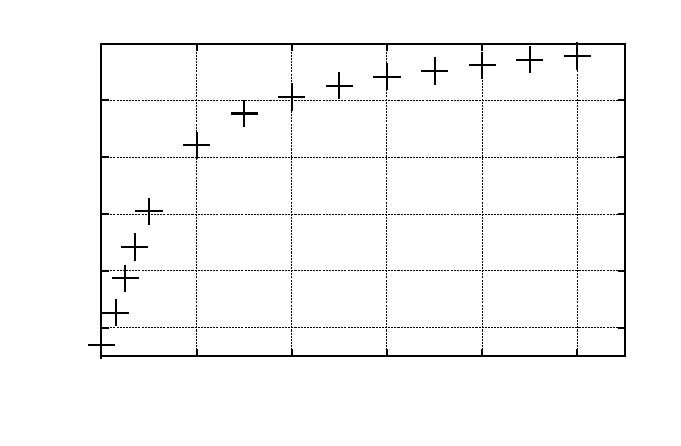
\includegraphics{prvni}}%
    \gplfronttext
  \end{picture}%
\endgroup

\caption{Závislost stejnosměrného napětí $U$ na filtrační kapacitě $C$}
\label{g:prvni}
\end{graph}


\begin{tabulka}[htbp]
\centering
\begin{tabular}{c|c}
$C$ (\si{\micro\farad}) & $U$ (\si{\volt}) \\ \hline
0 & \num{2.69(1)} \\
\num{0.3} & \num{3.26(1)} \\
\num{0.5} & \num{3.87(2)} \\
\num{0.7} & \num{4.42(3)} \\
1 & \num{5.05(3)} \\
2 & \num{6.21(3)} \\
3 & \num{6.77(4)} \\
4 & \num{7.06(4)} \\
5 & \num{7.26(4)} \\
6 & \num{7.42(4)} \\
7 & \num{7.52(4)} \\
8 & \num{7.62(4)} \\
9 & \num{7.72(4)} \\
10 & \num{7.78(4)} \\
\end{tabular}
\caption{Závislost stejnosměrného napětí $U$ na filtrační kapacitě $C$}
\label{t:kapacita}
\end{tabulka}


Změřili jsme závislost filtrační kapacity $C$ potřebné k tomu, aby střídavá složka napětí tvořila \SI{1}{\volt} na odebíraném proudu $I_{SS}$.
Výsledky jsou v tabulce \ref{t:desetprocent} a grafu \ref{g:druhy}.
U kapacit uvádíme poslední číslici v řádu, ve kterém jsme ještě pozorovali rozdíl na osciloskopu, proto uvažujeme chybu $C$ približně \SI{1}{\percent}, od toho se odvíjí i chyba $\tau$.

\begin{graph}[htbp] 
\centering
% GNUPLOT: LaTeX picture with Postscript
\begingroup
  \makeatletter
  \providecommand\color[2][]{%
    \GenericError{(gnuplot) \space\space\space\@spaces}{%
      Package color not loaded in conjunction with
      terminal option `colourtext'%
    }{See the gnuplot documentation for explanation.%
    }{Either use 'blacktext' in gnuplot or load the package
      color.sty in LaTeX.}%
    \renewcommand\color[2][]{}%
  }%
  \providecommand\includegraphics[2][]{%
    \GenericError{(gnuplot) \space\space\space\@spaces}{%
      Package graphicx or graphics not loaded%
    }{See the gnuplot documentation for explanation.%
    }{The gnuplot epslatex terminal needs graphicx.sty or graphics.sty.}%
    \renewcommand\includegraphics[2][]{}%
  }%
  \providecommand\rotatebox[2]{#2}%
  \@ifundefined{ifGPcolor}{%
    \newif\ifGPcolor
    \GPcolorfalse
  }{}%
  \@ifundefined{ifGPblacktext}{%
    \newif\ifGPblacktext
    \GPblacktexttrue
  }{}%
  % define a \g@addto@macro without @ in the name:
  \let\gplgaddtomacro\g@addto@macro
  % define empty templates for all commands taking text:
  \gdef\gplbacktext{}%
  \gdef\gplfronttext{}%
  \makeatother
  \ifGPblacktext
    % no textcolor at all
    \def\colorrgb#1{}%
    \def\colorgray#1{}%
  \else
    % gray or color?
    \ifGPcolor
      \def\colorrgb#1{\color[rgb]{#1}}%
      \def\colorgray#1{\color[gray]{#1}}%
      \expandafter\def\csname LTw\endcsname{\color{white}}%
      \expandafter\def\csname LTb\endcsname{\color{black}}%
      \expandafter\def\csname LTa\endcsname{\color{black}}%
      \expandafter\def\csname LT0\endcsname{\color[rgb]{1,0,0}}%
      \expandafter\def\csname LT1\endcsname{\color[rgb]{0,1,0}}%
      \expandafter\def\csname LT2\endcsname{\color[rgb]{0,0,1}}%
      \expandafter\def\csname LT3\endcsname{\color[rgb]{1,0,1}}%
      \expandafter\def\csname LT4\endcsname{\color[rgb]{0,1,1}}%
      \expandafter\def\csname LT5\endcsname{\color[rgb]{1,1,0}}%
      \expandafter\def\csname LT6\endcsname{\color[rgb]{0,0,0}}%
      \expandafter\def\csname LT7\endcsname{\color[rgb]{1,0.3,0}}%
      \expandafter\def\csname LT8\endcsname{\color[rgb]{0.5,0.5,0.5}}%
    \else
      % gray
      \def\colorrgb#1{\color{black}}%
      \def\colorgray#1{\color[gray]{#1}}%
      \expandafter\def\csname LTw\endcsname{\color{white}}%
      \expandafter\def\csname LTb\endcsname{\color{black}}%
      \expandafter\def\csname LTa\endcsname{\color{black}}%
      \expandafter\def\csname LT0\endcsname{\color{black}}%
      \expandafter\def\csname LT1\endcsname{\color{black}}%
      \expandafter\def\csname LT2\endcsname{\color{black}}%
      \expandafter\def\csname LT3\endcsname{\color{black}}%
      \expandafter\def\csname LT4\endcsname{\color{black}}%
      \expandafter\def\csname LT5\endcsname{\color{black}}%
      \expandafter\def\csname LT6\endcsname{\color{black}}%
      \expandafter\def\csname LT7\endcsname{\color{black}}%
      \expandafter\def\csname LT8\endcsname{\color{black}}%
    \fi
  \fi
  \setlength{\unitlength}{0.0500bp}%
  \begin{picture}(6236.00,3968.00)%
    \gplgaddtomacro\gplbacktext{%
      \csname LTb\endcsname%
      \put(814,704){\makebox(0,0)[r]{\strut{} 0}}%
      \csname LTb\endcsname%
      \put(814,1104){\makebox(0,0)[r]{\strut{} 2}}%
      \csname LTb\endcsname%
      \put(814,1504){\makebox(0,0)[r]{\strut{} 4}}%
      \csname LTb\endcsname%
      \put(814,1904){\makebox(0,0)[r]{\strut{} 6}}%
      \csname LTb\endcsname%
      \put(814,2303){\makebox(0,0)[r]{\strut{} 8}}%
      \csname LTb\endcsname%
      \put(814,2703){\makebox(0,0)[r]{\strut{} 10}}%
      \csname LTb\endcsname%
      \put(814,3103){\makebox(0,0)[r]{\strut{} 12}}%
      \csname LTb\endcsname%
      \put(814,3503){\makebox(0,0)[r]{\strut{} 14}}%
      \csname LTb\endcsname%
      \put(946,484){\makebox(0,0){\strut{} 0}}%
      \csname LTb\endcsname%
      \put(1519,484){\makebox(0,0){\strut{} 0.1}}%
      \csname LTb\endcsname%
      \put(2093,484){\makebox(0,0){\strut{} 0.2}}%
      \csname LTb\endcsname%
      \put(2666,484){\makebox(0,0){\strut{} 0.3}}%
      \csname LTb\endcsname%
      \put(3239,484){\makebox(0,0){\strut{} 0.4}}%
      \csname LTb\endcsname%
      \put(3812,484){\makebox(0,0){\strut{} 0.5}}%
      \csname LTb\endcsname%
      \put(4386,484){\makebox(0,0){\strut{} 0.6}}%
      \csname LTb\endcsname%
      \put(4959,484){\makebox(0,0){\strut{} 0.7}}%
      \put(5091,704){\makebox(0,0)[l]{\strut{} 0}}%
      \put(5091,1104){\makebox(0,0)[l]{\strut{} 2}}%
      \put(5091,1504){\makebox(0,0)[l]{\strut{} 4}}%
      \put(5091,1904){\makebox(0,0)[l]{\strut{} 6}}%
      \put(5091,2303){\makebox(0,0)[l]{\strut{} 8}}%
      \put(5091,2703){\makebox(0,0)[l]{\strut{} 10}}%
      \put(5091,3103){\makebox(0,0)[l]{\strut{} 12}}%
      \put(5091,3503){\makebox(0,0)[l]{\strut{} 14}}%
      \put(176,2203){\rotatebox{-270}{\makebox(0,0){\strut{}$C$ (\si{\micro\farad})}}}%
      \put(5728,2203){\rotatebox{-270}{\makebox(0,0){\strut{}$\tau$ (\SI{e-2}{\second})}}}%
      \put(2952,154){\makebox(0,0){\strut{}$I$ (\si{\milli\ampere})}}%
      \csname LT0\endcsname%
      \put(3239,1704){\rotatebox{30}{\makebox(0,0)[l]{\strut{}$C(\si{\micro\farad})=\num{17.0} \cdot I(\si{\milli\ampere})$}}}%
      \csname LT0\endcsname%
      \put(1519,3103){\makebox(0,0)[l]{\strut{}$\tau = \SI{13.7e-2}{\second}$}}%
    }%
    \gplgaddtomacro\gplfronttext{%
      \csname LTb\endcsname%
      \put(3972,1357){\makebox(0,0)[r]{\strut{}$C$}}%
      \csname LTb\endcsname%
      \put(3972,964){\makebox(0,0)[r]{\strut{}$\tau$}}%
    }%
    \gplbacktext
    \put(0,0){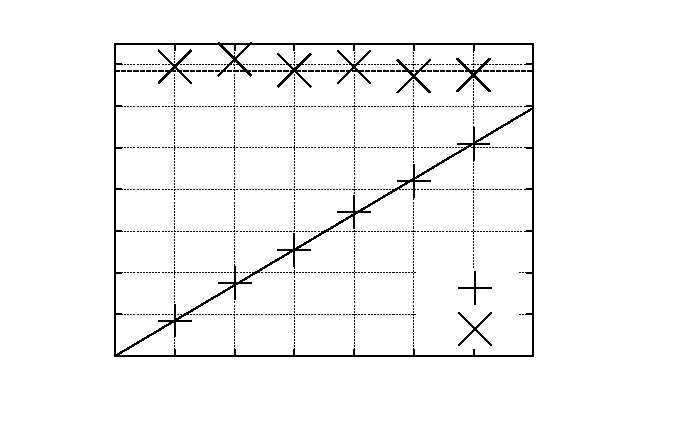
\includegraphics{druhy}}%
    \gplfronttext
  \end{picture}%
\endgroup

\caption{Závislost filtrační kapacity $C$ potřebné k tomu, aby střídavá složka napětí tvořila \SI{1}{\volt} špičkové hodnoty, na odebíraném proudu $I_{SS}$}
\label{g:druhy}
\end{graph}

\begin{tabulka}[htbp]
\centering
\begin{tabular}{c|c|c|c}
$I_{SS}$ (\si{\milli\ampere}) & $R_Z$ (\si{\kilo\ohm}) & $C$ (\si{\micro\farad}) & $\tau$ (\SI{e-2}{\second}) \\ \hline

\num{0.10} & \num{81.7} & \num{1.7} & \num{13.9(2)} \\
\num{0.20} & \num{40.7} & \num{3.5} & \num{14.2(2)} \\
\num{0.30} & \num{26.9} & \num{5.1} & \num{13.7(2)} \\
\num{0.40} & \num{20.1} & \num{6.9} & \num{13.9(2)} \\
\num{0.50} & \num{16.0} & \num{8.4} & \num{13.4(2)} \\
\num{0.60} & \num{13.2} & \num{10.2} & \num{13.5(2)} \\
\end{tabular}
\caption{Závislost filtrační kapacity $C$ potřebné k tomu, aby střídavá složka napětí tvořila \SI{1}{\volt} špičkové hodnoty, na odebíraném proudu $I_{SS}$}
\label{t:desetprocent}
\end{tabulka}

Statisticky zpracujeme hodnoty $\tau$ v tabulce \ref{t:desetprocent} a dostáváme $\tau =\SI{0.137(4)}{\second}$.

\subsection*{Charakteristiky diod}

Na osciloskopu jsme zobrazili V-A charakteristiku vakuové diody \textbf{EZ81} a Zenerovy diody \textbf{KZ703}.
Charakteristiky jsou načtrtnuty v přiloženém záznamu z měření.
Napětí na vakuové diodě při proudu \SI{20}{\milli\ampere} jsme odhadli \SI{6.4(3)}{\volt}.
Na Zenerově diodě jsme ho odhadli \SI{0.64(4)}{\volt}.
U Zenerovy diody jsme napětí odhadovali při jiném měřítku, než ve kterém je načtrnut výstup osciloskopu.
Odhadli jsme Zenerovo napětí \SI{6.8(1)}{\volt}.